\section{Diagrama de Classe com Estruturas de Dados e com ORM}
Partindo do Modelo de Domínio e dos diagramas de sequência de sistema e subsistemas, procedemos à definição do diagrama de classes, numa primeira fase, usando estruturas de dados do Java. O processo de construção foi iterativo e realizado, de certa forma, paralelamente ao desenvolvimento dos diagramas de sequência de implementação. De seguida, apresenta-se uma primeira versão do diagrama, sem implementação de persistência. Posteriormente, é apresentada a versão com DAOs. 
\begin{center}
 	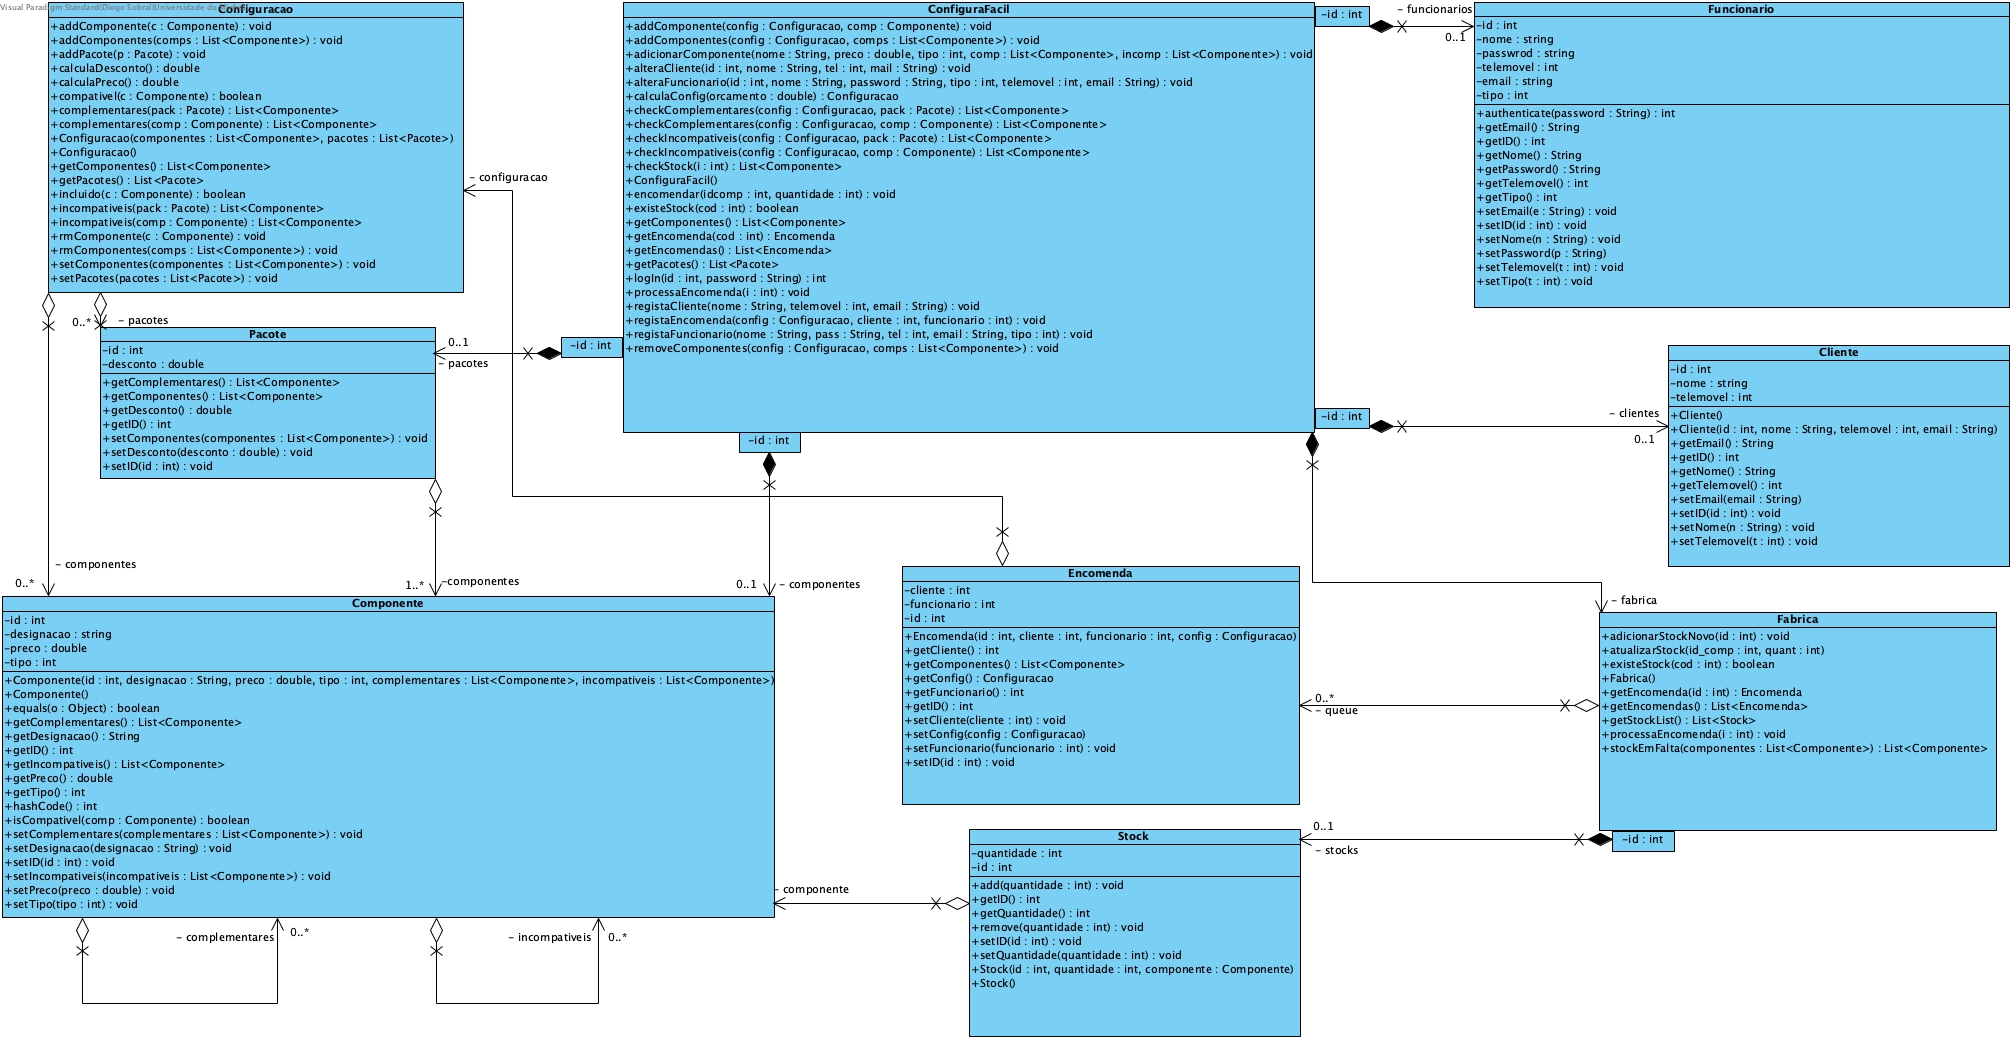
\includegraphics[width=6in]{VPP/Diagrama_de_Classes.jpg}
\end{center}

\newpage
O passo seguinte foi, tendo em conta o ORM, decidir quais as classes que deveriam persistir. Assim, pela nossa análise, selecionamos as seguintes classes: Cliente, Funcionário, Encomenda, Componente, Pacote e Stock. Deste modo, obtivemos o seguinte diagrama de classes:

\begin{center}
 	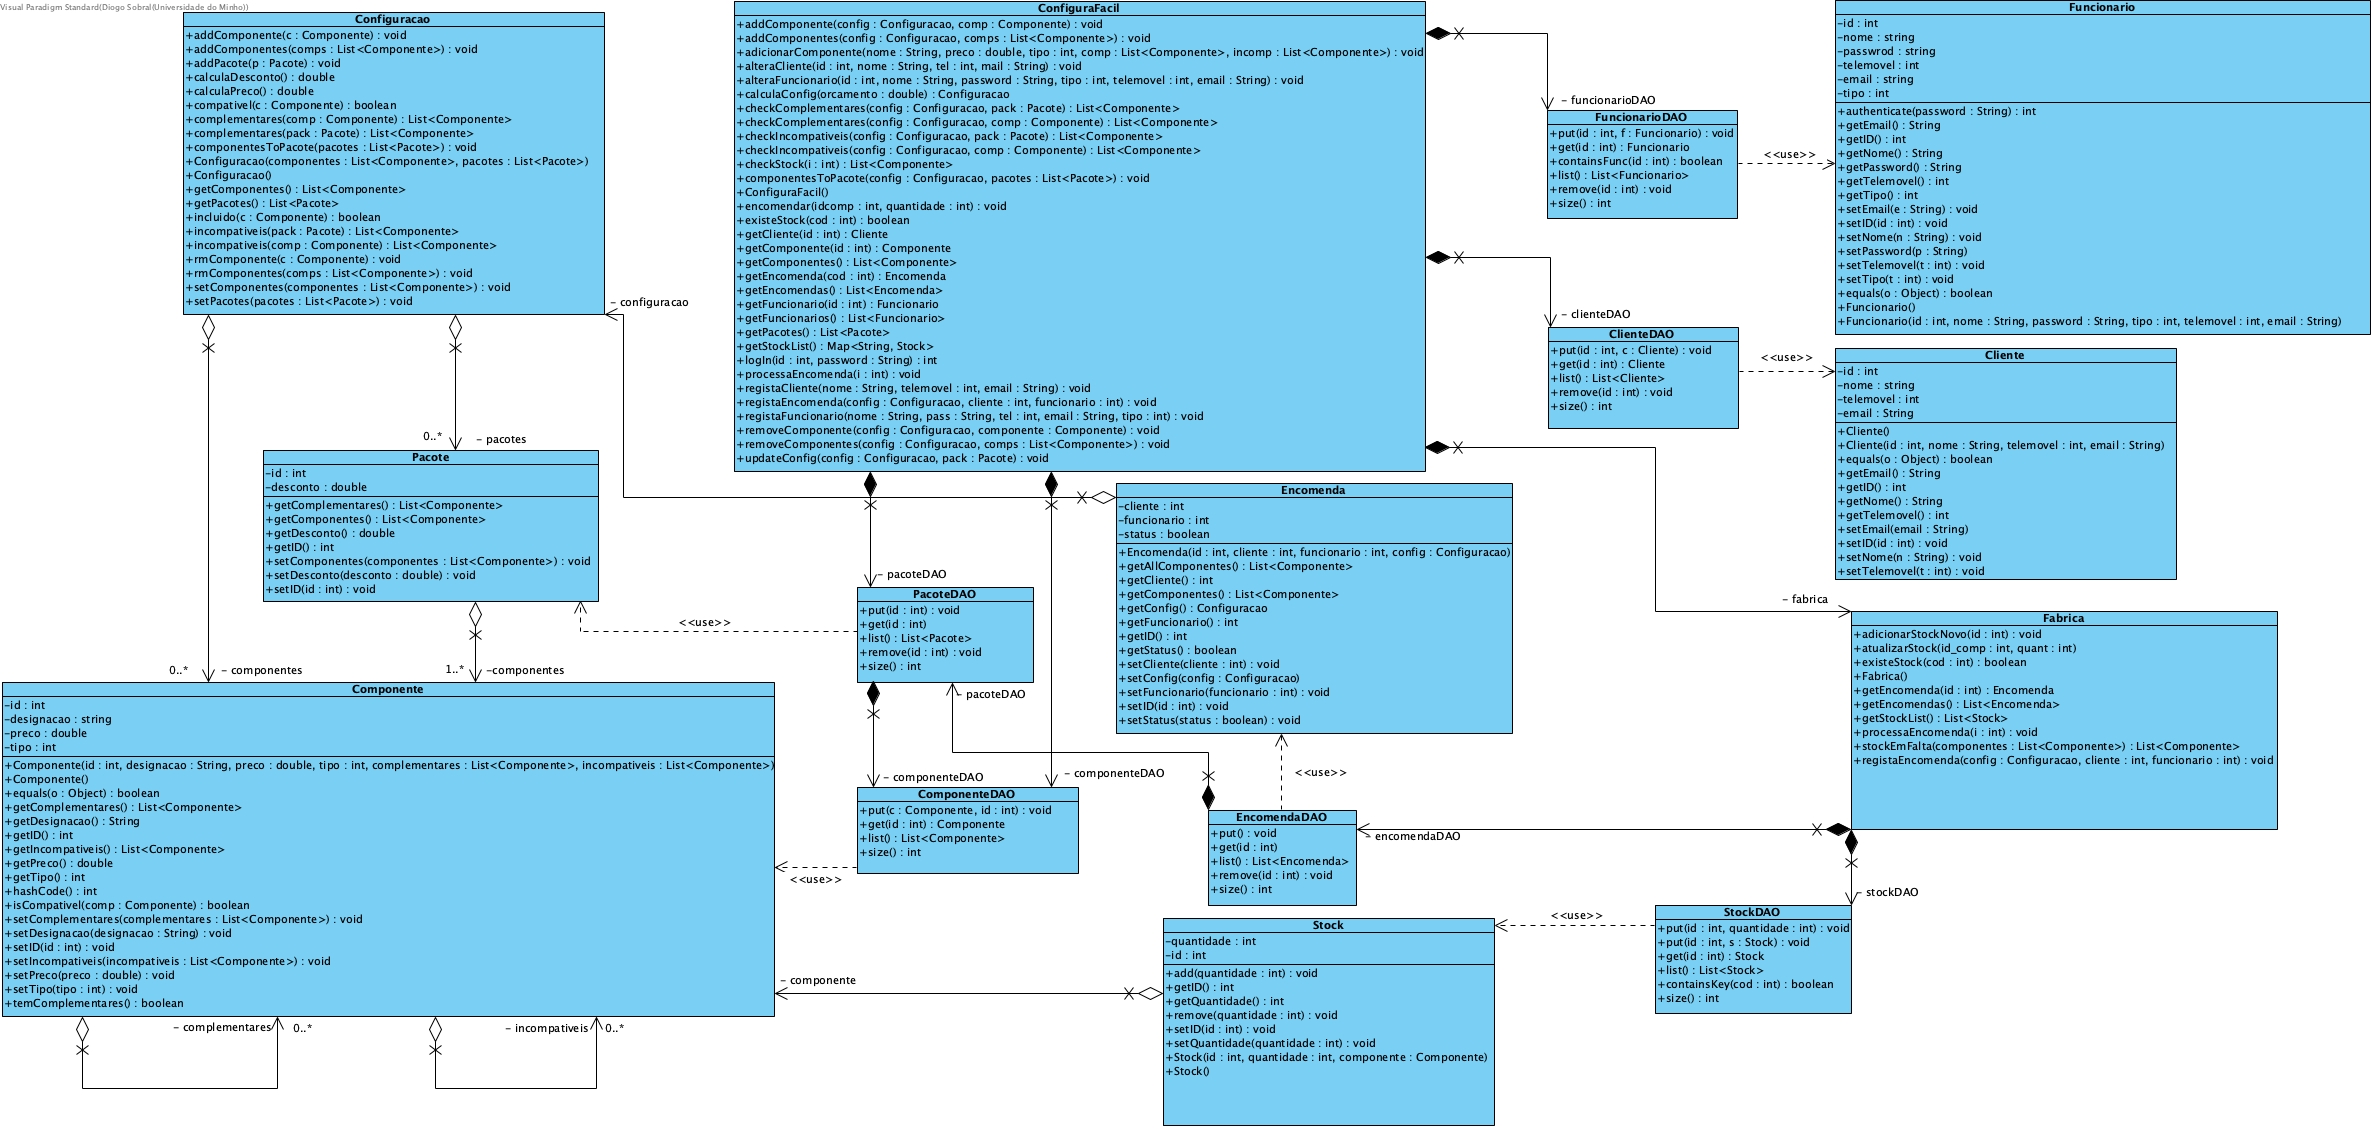
\includegraphics[width=6in]{VPP/diagramadao.jpg}
\end{center}
\newpage
